%%%%%%%%%%%%%%%%%%%%%%%%%%%%%%%%%%%%%%%%%%%%%%%%%%%%%%%%%%%%%%%%%%%%
%% UNSW SENG2020 2012S2 GROUP 6 REPORT TEMPLATE
%% CREATED BY VINCENT WONG
%%%%%%%%%%%%%%%%%%%%%%%%%%%%%%%%%%%%%%%%%%%%%%%%%%%%%%%%%%%%%%%%%%%%

\documentclass[a4paper]{article}
\usepackage[margin=1.5in]{geometry}
%\usepackage{a4wide}
\usepackage{longtable}
%\usepackage[normalem]{ulem}     %% gives strikeout capability with \sout{}
\usepackage{graphicx}
\usepackage{float}
\usepackage[usenames,dvipsnames]{color}
\RequirePackage{bsymb,b2latex}
%%%%%%%%%%%%%%%%%%%%%%%%%%%%%%%%%%%%%%%%%%%%%%%%%%%%%%%%%%%%%%%%%%%%%
%% DOCUMENT MACROS -- DO NOT DELETE


\begin{document}

%%%%%%%%%%%%%%%%%%%%%%%%%%%%%%%%%%%%%%%%%%%%%%%%%%%%%%%%%%%%%%%%%%%%%
%% TITLE PAGE
\thispagestyle{empty}      % turn off page numbering
\begin{center}
\Large\textbf{$\odot\int$ Sale} %%\odot \int Sale

\Large\textbf{Design Report}

%%%% MAKE SURE YOU SPECIFY YOUR GROUP NUMBER
\bigskip\large\textbf{Group Number: 06}
\end{center}

\vspace*{16.5cm}
\begin{tabular}{|l|l|}
  \hline
  Version         & 1.0\\\hline
  Print Date      & 15/09/2012 13:37\\\hline
  Release Date    & 15/09/2012\\\hline
  Release State   & Final\\\hline
  Approval State  & Pending\\\hline
  Approved by     & Chris, Dylan, Lasath, Vincent\\\hline
  Prepared by     & Chris, Dylan, Lasath, Vincent\\\hline
  Reviewed by     & Chris, Dylan, Lasath, Vincent\\\hline
  Confidentiality Category  & Public\\\hline
\end{tabular}
\pagebreak

%%%%%%%%%%%%%%%%%%%%%%%%%%%%%%%%%%%%%%%%%%%%%%%%%%%%%%%%%%%%%%%%%%%%%
%% REVISION CONTROL PAGE
\thispagestyle{plain}     % Turn on page numbering
\setcounter{page}{1}      % set page number counter
\renewcommand{\thepage}{\roman{page}}  % set page number to roman

\noindent{\Large\textbf{Document Revision Control}}\\[2ex]
\begin{tabular}{|l|l|l|l|}
  \hline
  Version & Date & Authors & Summary of Changes\\\hline\hline
  0.1 & 03/08/2012     &    Vincent     &    Created initial report               \\\hline
   0.2 & 03/08/2012     &    Lasath     &    Added Architecture section               \\\hline
    0.9 & 14/08/2012     &    ALL     &    Added in rest               \\\hline
 
\end{tabular}

\pagebreak

%%%%%%%%%%%%%%%%%%%%%%%%%%%%%%%%%%%%%%%%%%%%%%%%%%%%%%%%%%%%%%%%%%%%%
%% TABLE OF CONTENTS AND FIGURES

\tableofcontents
\pagebreak


%%%%%%%%%%%%%%%%%%%%%%%%%%%%%%%%%%%%%%%%%%%%%%%%%%%%%%%%%%%%%%%%%%%%%
%% MAIN DOCUMENT
\setcounter{page}{1}     % Set page number counter
\renewcommand{\thepage}{\arabic{page}}  % print page number as arabic

%%%%%%%%%%%%%%  THIS IS WHERE YOU PUT YOUR CONTENT %%%%%%%%%%%%%%%%%%

\section{Overview}
The Point of Sale/Warehouse System (PosWare) is designed to be a simple yet sophisticated system that provides extensive sales and logistics management functionality to all kinds of businesses from large to small. 
\\\\
The system will be a distributed system which has various terminals and user interfaces allowing multiple actors in different locations within the store to use the system concurrently. It will also be scalable to suit the needs of different sizes of business, as it can handle the complexity of large chain businesses, while remaining cost effective for small independent stores.
\\\\
The system will incorporate 3 different terminal and user interface designs. This includes the cashier UI, the stock controllers UI and manager UI. They all provide specific layout designed to maximise the efficiency and ease of use for the targeted actor. We have chosen to utilise a prototyping approach in the design of our UI as we constantly release and refine previews of the system based on user feedback. 
\\\\
As the system is designed to suit different businesses, the clients will have an option of choosing their ideal combination of servers and terminals to suite their budgetary needs. They will also be able to opt in for various data redundancy programs such as offsite backups and automatic archiving as they see fit.
\\\\
The majority of the functionality has been modelled using EventB. The backend will stick as close to the model as possible since we understood that the model was constructed to meet the customers requirements, and is internally consistent. The transition is a reasonably straightforward process as outlined in detail later on this document.
\\\\
The following report will outline our final version of our requirements (see appendix) and our complete use case diagram. The report will also provide brief description of the use cases and mapping the various use case to our EventB model in detail. Following this, the report will explain the architecture of our system and the formal specification. Finally our report will provide quick insight into our proposed graphical user interface and the features which our system has to offer.
\pagebreak

\section{Design Considerations}
Our system has to be able to be deployed across multiple machines to suit the needs of medium to large businesses. This allows for cashiers and stock controllers to be in separate locations while working on the same system and also allows multiple cashiers/customers to be active at once (as stated by requirement PD-2.1.1.1). However this does contrast to the capabilities of EventB, which models a single system with a state and purely atomic operations and would be difficult to implement whilst spread over multiple machines.
\\\\
In an attempt to stick as close to the model as possible, we decided to store all state in a database. Since all machines can access this database it essentially allows for a single shared state between the machines.
\\\\
Events were converted into methods (as explained in detail in section 4.0), which will run in a central server. Since all state is maintained within the database, it is unnecessary for these methods/classes to maintain any local state. If fact, doing so is likely to cause unintended consequences or extra side effects. In order to keep these methods atomic, to match model events, they were restricted to one database update query per method (except during rare special circumstances) .
\\\\
Keeping the methods in classes which maintain no state on themselves during execution, whilst allowing us to match the model events, also caused another advantage; they can be executed on different machines. This will allow for good scalability in case of large businesses with lots of machines, they can merely have multiple of servers with distributed load balancing. 
\\\\
This leaves most of the machines as thin clients since they will only need to perform enquiry services rather than individual processing. At this time we are considering making these clients web based for the ease of deployment. 
\\\\
The system will have a backup servers in case issues arise from the system in-store. All the data will be backed up offsite on the users choice of cloud storage provider. The system will be made such that if any issues arise with the onsite servers, requests can be redirected to offsite servers temporarily while the issue gets resolved.The terminals can be replaced if broken as our system has no reliance on the terminal for the system functionality. 
\\\\
We will have 3 key types of user interfaces in this system and each will run on thin clients. These include the Cashiers UI which will be run on the cash registers, Stock controller UI which will be run on back room machines, and the manager UI which can be run anywhere throughout the system. 
\\\\
We also have pay particular attention during the design of the user interface such that it fits into the philosophy we set for this system - simple yet powerful. The user interface should be easy to understand as users will need to be able to use our system without any prior knowledge or reading any sort of user manual. The layout of the system should be clear and straightforward, whilst having messages across the screen guiding users on how to use the system. As stated by requirement PD-4.2.2, the user interface should also have a dedicated help button each screen to aid users in using the system.
\pagebreak

\section{Class Overview }
As explained above, our Stock\_Control\_RX machine was decomposed into several instances of MVC which makes up the core of our system. However for simplicity, they will be referred to as single classes in this section. 
\\\\
Product forms the primary subject of the majority of our requirements and our EventB model. Each instance represents a physical product line sold in store, just as the PRODUCT set from Stock\_Ctx did. A product stores information required to uniquely identify itself as well as cosmetic (non-functional) details to display to the user [PD-1.1.{2,3,4}]. 
However, products need have to have much more data to fulfil most requirements. Thus they are linked to many other objects including suppliers, orders, and sales.
\\\\
As shown in requirements DN-1.1, … , they need to have a stock level associated with them for each stock location. Like the product levels variable in the model, each product instance has an associated stock level with them through stock location. 
\\\\
Each product also has an associated Supplier in order to fulfil requirements PD-1.4.1. Each supplier instance represents an external supplier. They are a subject of Stock Orders, and their primary role is to interact with the system to automatically place a purchase order. Since this step is very hard to model in EventB, it was deemed pointless to model them at all.
\\\\
The rest of our classes are mainly involved with the sales of items and their payments. A dedicated sale class allows us to have many sale items as well as multiple payment transaction for each purchase. The sale class also interact with users which includes both customer and a system user. These combined allow us to meet all the requirements, within our system by directly relating to your EventB.
\\\\
The workers and the customers in the system are represented as users, and all the attributes provide the features that were required by our system. It allowed us to create and edit the users as well as apply discounts for both staff and customers, as described by our requirements for this system.
\pagebreak

\section{Class Diagram}
\begin{figure}[h]
\centering
  \hspace*{-0.3in}
  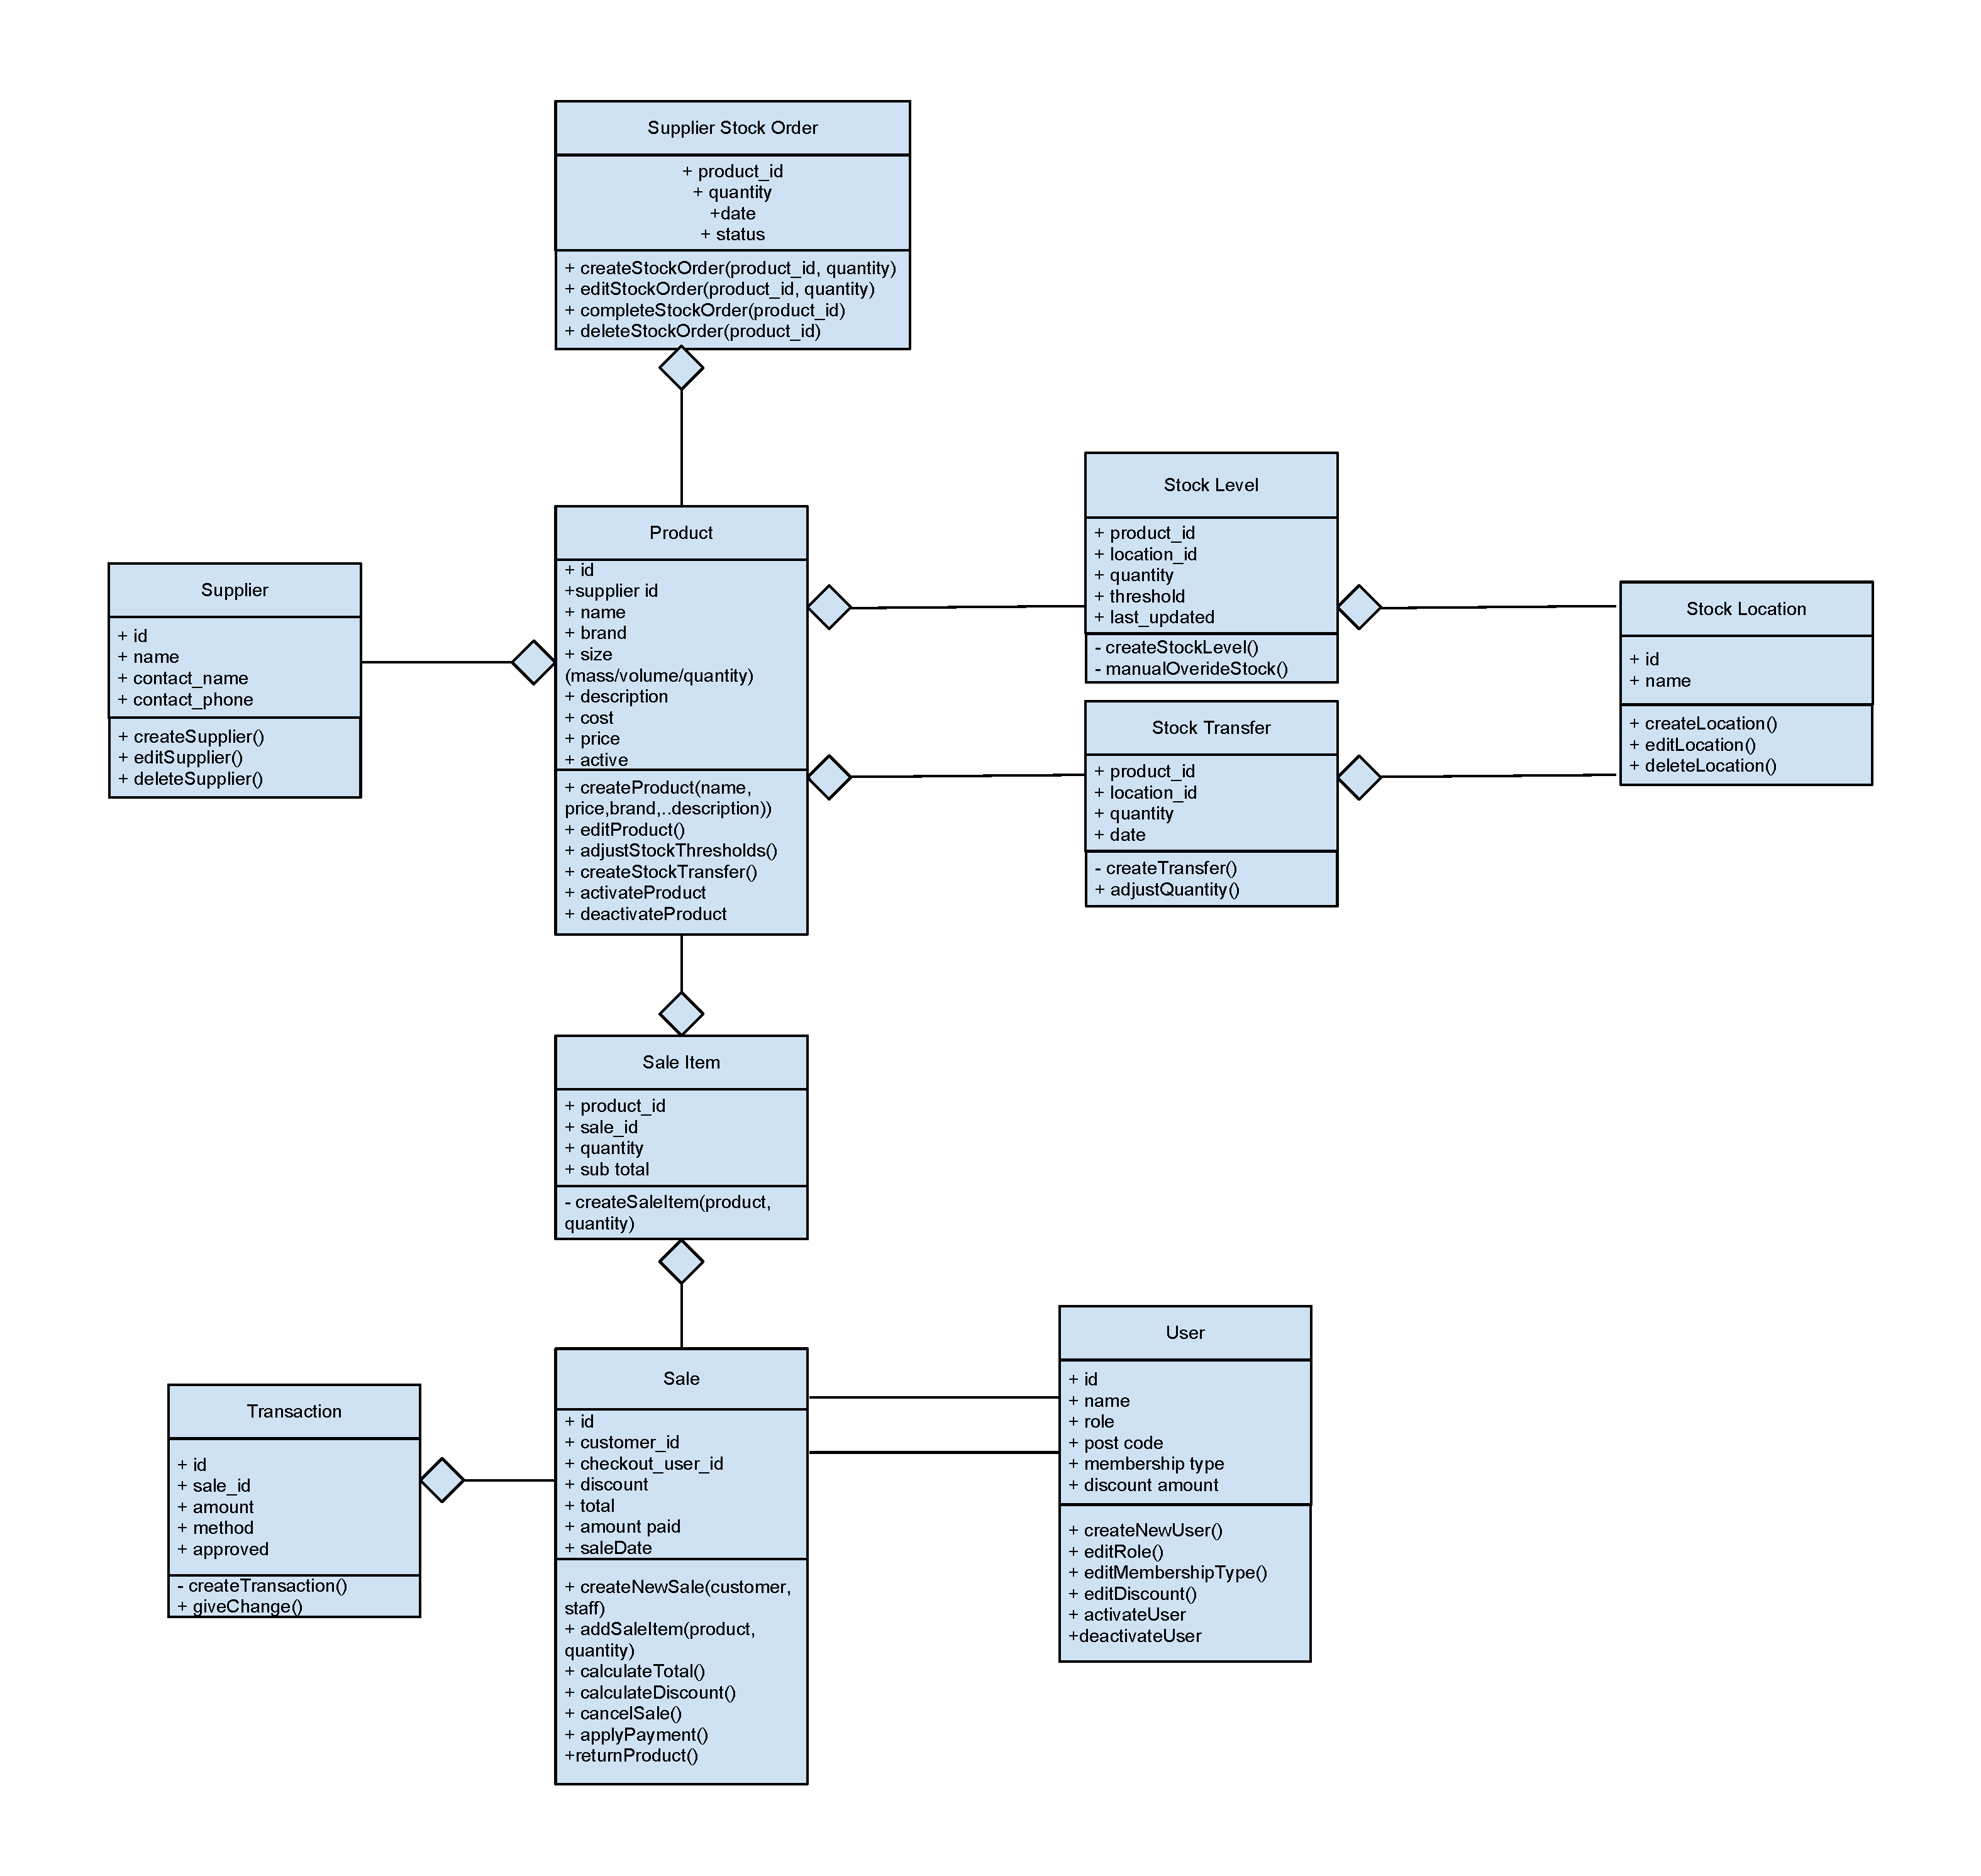
\includegraphics[scale=0.3]{ClassDiagram.pdf}
	\caption{Class diagram designed for superheroes}
\end{figure}

\pagebreak

\section{EventB to Class Mapping}
Last semester we modelled our requirements for our point of sales system in EventB, this enabled us to determine whether the requirements we had devised were internally consistent. It also ensures us that our completed system will meet all the set requirements and also be highly effective.
\\\\
Within our EventB model, most of the sets defined in our contexts were converted classes. All variables that map sets defined in the contexts to another set or value were converted into attributes within those classes. Additional attributes were added to the classes for metadata as they were pointless to model in EventB. These consisted of non-functional cosmetic metadata, such as description and name attributes, to allow for added to ease of use for the customer.
\\\\
The main class was supplier stock order which dealt with all the attributes related to the stock orders, while the class methods were of direct correlation to the events. The attributes extracted from the invariants were product\_id, quantity, status and date. The date attribute was added as metadata to provide ease of use sorting for the end-user. Events that involved ordering were converted to methods with a one to one correlation, although the events which dealt with updating the status and editing the order were merged into one method called update order. Cancel and delete were equivalent. This all represents our requirement DN - 1.4
\\\\
The two key variables were orders \(orders ∈ activeProducts ⇸ ℕ1;\) and\\\\ \(orderStatus orderStatus ∈ activeProducts ⇸ ORDER_STATUS;\).\\\\
The first shows how an order involved a product and a quantity, the second showed how orders had a status, which were implicitly stated by [DN-1.4] and explicitly by [DN-3.1]. These generated attributes for the order class quantity and status. The invariant \(∀p · p ∈ activeProducts ∧ p ∈ dom(orders) ⇒ p ∈ dom(orderStatus);\) clearly showed the link between products and orders status and the need for the status attribute.
\\\\
This refinement StockControl\_R1 added numerous events which dealt with the creation of stock orders to suppliers and editing of orders. The NewOrder event took three parameters this was converted to a method called createStockOrder in the class, it did not take the additional user parameter as this will be handled by the authentication controller in our system [PD-1.4.1]. EditOrder was also nearly a direct conversion from the event-b model into the class diagram as a method named EditStockOrder which was similar to new order in which it didn't take a user as this is handled elsewhere in the system. [PD-1.4.3]
\\\\
UpdateOrder and CompleteOrder, were events in the model were merged into one combined method in our class diagram named completeStockOrder, and there were no major changes in the merge. There is no direct requirement for completing a stock order, as tracking orders implies that the system will be able to complete an order. The last event from this refinement was CancelOrder which was changed to a method in the supplierstockorder class called deletestockorder. [PD-1.4.3]
\\\\
The initial refinements which dealt with the generalisation of products was decomposed into both the invariants which defined attributes and the methods. The product class was generated, and as stated in previous sections all attributes were either had a direct relation with the EventB model, or were added as metadata in our class to provide the ease of use for the client. The events; NewProduct [PD-1.1.2], UpdateProduct [PD-1.1.3], ActivateProduct, DeactivateProduct[PD-1.1.4 combined with PD-3.1.2 and PD-2.2.1], were added as methods to the class. The only change was the renaming of update to edit. Additionally a few events which were directly related to stock levels and products were added as methods to the products. This included creating a stock transfer and adjusting the thresholds. Overall this correlated directly to our EventB representation of products, with a large number of methods that were wrappers for calling another method on one of its relations.
\\\\
The main variable that dealt with products is product price \(productprice ∈ products → ℕ;\) which brought about the price attribute of the product class. The active attribute of the class was derived from the activeProducts variable, which is a subset of products \(activeProducts ⊆ products;\), This subset was used to check whether the products were active or not and hence is a boolean. The  rest of the attributes of the product class were added as a form of metadata, that enables ease of use for user and also adds sorting abilities based on the metadata.
\\\\
The base machine included a NewProduct [PD-1.1.2] event which was converted to a method named createProduct, on the most part the attributes remained the same except that the method included additional parameters for the metadata. Another event in the model was UpdateProduct  [PD-1.1.3] which was used to change the products price, in its current state the  method in the class is called editProduct and hence this also reflects the increase in parameters due to the attributes. The activateProduct and deactivateProduct events were converted into methods with the same name and instead of altering which set it is. The method will just enable and disable the boolean attribute.
\\\\
The stock level class mainly came about from the function in our EventB model which were used to show the relation between the products and stock\_locations. This invariant \(productlevels ∈ products →(STOCK_LOCATION → ℕ) \) was the cause for the main attribute of the class, although additional attributes were added as a form of metadata. The main events which were ported to this class as methods were the events to do with directly altering product levels, ie setProductLevel[PD-1.1.1], removeStock[PD-1.1.1] and addStock [PD-1.1.1]. These are all merged into a private manual override method.
\\\\
The two main variables which gave rise to the attributes of the stock\_level class were product\_threshold, which was \(productthreshold ∈ products → (STOCK_LOCATION → ℕ) \) [PD-1.4.4] and product which was \( productlevels ∈ products →(STOCK_LOCATION → ℕ) \) [PD-1.1.3]. They respectively brought about the threshold and levels attributes of the class. In this case last\_updated was added as a metadata attribute so that the there is added ease of use for the user. 
\\\\
The two methods of this class were createStockLevel[PD-1.1.2] and manualOverrideStockLevel [PD-1.1.3], these were derived from the combination of many events in our refinement so that we could call the adjustments in the stock levels from the product class. The main events which were merged into these were, AddStock, RemoveStock and SetProductLevel, this was easily done as addStock and removeStock could be derived from the setProductLevel. 
\\\\
Another addition to the class was that of its abilities to set the products threshold through this manual override. This was useful since the EventB model of the two sets were defined by almost identical invariants. This is used by the product class once again to adjust the products threshold [PD-1.4.4].
\\\\
Within our event-b model we had two sets for both the members and users, as it provided the easiest form of modelling our solution at the time. However when we begun to work on our class diagram we could see that they were both virtually the same and any attributes that were only in one of them could be consider as metadata for the other. Hence we decided to merge both the member and user in the class diagram to the user class, all the attributes either came from the invariants which linked to either user or members to certain sets. The NewMember [PD-2.4.2] and NewUser were converted into the createUserMethod of our class, the editRole method had a direct correlation to to editUserPrivileges [4.1.3], but the only change that will actually occur in the method is that there is now an option for the role of basic member. The editMemberType and editDiscount methods were used to replace the setMemberDiscount, removeCredit and addCredit events in our model.
\\\\
In the first refinement of our EventB machine we added the user set and user privileges, this was used to create the user class. The userPrivileges [PD-4.1.2] invariant \(userPrivileges ∈ users → USER_PRIVILEGE; \) was used to create the attribute of role, which will be used to contain a value which defines there user\_privilege. There were other attributes which were derived from the fourth refinement of the model these include memberDiscounts [2.4.1] invariant \(memberDiscounts ∈ members → 1‥100; \), which resulted in the membershipType and discountAmount attributes of the class.
\\\\
Overall it is evident that although they were modelled independently in EventB, users and members can be represented by the same class in our class diagram. This is because they are both essentially similar actors in the system with similar metadata, and hence they should be the same class.
\\\\
Our EventB model had the notion of carts and receipts, during the design process we decided that the best way to convert it into class diagram was to split these into two objects: one of which was a the sale class, and the other sale item class. The newCart event was added to the sale class as a method named create new sale, similarly addProductToCart was replaced by a method with the name add sale item, and finally calculateTotalCart [PD-2.2.3], was just simply shortened and added as a method name calculate total. All invariants involving sales were also added as attributes, although a few additional attributes were added as a form of metadata. CancelCheckout from our event-b model was also renamed as a method of sale and it was renamed to cancelSale, but still provided the same functionality and consistency. Additionally the returnProduct  event was added to this class as a method to ensure that integrity was kept between our design and our event b model.
\\\\
The final refinement of the context evolved the notion of a [PD-2.1.2] \(CART = CART = PRODUCT ⇸ ℕ; \), this was used to modelled in our class diagram as a SaleItem, its attributes are directly derived from the definition with product being the product\_id and the number being the quantity. The next immediate class that was derived from our refinement was that of sales, this was derived from the invariant \(carts ∈ members ⇸ CART; \). The customer\_id attribute was derived from the definition of the invariant which had a members and return a cart i.e. a sale item. The cartTotal invariant  was the invariant behind the total attribute of the sale, similarly the discountedCartTotal  was converted from the model into the discount, although this wasn't a direct correlation, the discountedCartTotal [PD-2.1.3] from the model can be calculated in the class from the total-discount. SaleDate was just added as a form of metadata to increase ease of use  for the user. 
\\\\
The amount\_paid class attribute was not modelled for each cart in the EventB model due to limitations in rodin, so it was used as a global attribute in the model that was reset at the end of each purchase. However in the design of our class we stored it as a local attribute. This will allow us to have multiple purchases happening simultaneously.
\\\\
The newCart event from our model was converted directly into a method named createSaleItem, it takes in the same parameters as the model including a customer i.e. member and staff use. The addProductToCart event was converted to the the method createSaleItem, and the methods took the exact same parameters as the EventB model. The calculateTotal method was derived from the CalculateTotalCart [PD-2.1.3] event from the model that was created last semester.  The last event from our model was that was added to this class was the cancelCheckout event, this had a direct relation to a new method named in the class and the only difference was that of it being renamed to cancelSale.
\\\\
The EventB refinement which involved paying for a cart [PD-2.3.1] were turned into the payment classes. The way in which multiple payments could be used in the EventB model was replicated so sales could have multiple payments. All the events for paying were basically converted to the one method, which was create payment the only difference is that the the create payment method would be called with different parameters. The attributes stored in the class are basically only used as metadata, and provide no extra validity to the EventB model but just focused on adding functionality for the end user. The GiveChangeCash event from our model was directly changed to a method giveChange in of the transaction class and allows for payments to pay with larger amounts and receive change.
\\\\
We decided to implement payments [PD-2.3.1], with a separate class, although in our EventB model these weren't represented as an a set of payments due to the fact that the EventB does not handle concurrency well. But this adds ease of use for the customers as it enables them to apply different types of payments  across one purchase. 
\\\\
The attributes of the transaction [PD-2.1.3 and PD-2.3.1] class are mainly derived from the temporary values of the that were used in the payForCartCash, payForCartOtherPayment, payCash. Combined with the sales class they are able to directly relate to the amountDue, paidAmount and change. The methods of the class are generated by merging all the payForCart events.
\\\\
These events from our EventB model are not directly modelled in our class diagram as they do not specifically involve the persistent data, and hence would be used in the transaction controller. 
\\\\
The MovedReturnedStock event was also directly translated into a method. The event is concerned with the movement of stock when a returned item causes a location to exceed it stock threshold.
\pagebreak

\section{EventB Events to Methods}
In general all our events are directly converted to the methods. The parameters more often than not remained consistent, as described above, with minor changes in the naming of the attributes. The methods in each the classes will be explained below though generally all the methods derived from events in our model which requires authentication will have a check which the authorisation controller which is explained below in our mvs and architecture description.
\\\\
\subsection{PRODUCT}
{\bf + createProduct(name, price,brand,..description))}
All of the methods of the products, were derived from event b methods as explained in the previous section. The createProduct method was derived from the new product event, in this event there were guards to check that the product did not already exist, this will be most likely handled by the method coding providing an if statement if a search for the product returned a null result then it would proceed. The other checks on parameters such as that the price is positive will also be handled by if statements or conditional branching to handle the invalid input. 
\\\\
{\bf + editProduct()}
The editProduct method was derived from update product and hence as explained above inherits its parameters with minimal changes. The guards of the event are quite simple and will just be used in the method to verify that the product being edited is a valid product, this is handled by the programming language we have decided to use as it is impossible to call this method on a null object. all other attributes will be verified by the same rules laid out by the guards
\\\\
{\bf + adjustStockThresholds()}
The adjustStockThresholds method was derived from Set product threshold. In this method there are guards to check if the product exist, and if the floor, back room and warehouse exists as well. It also makes sure that the amount of stock is higher or equal to the new threshold that the user is currently setting. This is directly mapped to the methods as there will be if statements checking if these guards are passed but enabling the user to actually adjust the stock threshold. 
\\\\
{\bf + activateProduct}
The activate product method was a direct conversion of the event-b model, it will take in the same parameters. The method had minimal guards, these will be converted into the code through the use of conditions before changing the attribute within the class. The event represents the movement of a product into the active products set. 
\\\\
{\bf + deactivateProduct(product)}
Deactivate product accomplishes the functional equivalent of the deactivateProduct event. Its guards were simply that the product exists and that it wasn't already deactivated. This method will only be presented to the user if the above conditions hold, however it will also verify it before taking any action. The event moved the product from the activeProducts set to the products set. Since that set was only used for an inclusivity check, it was replaced by a boolean attribute in the code (as explained above). The method achieves the same result by setting that attribute to false. 
\\\\
\subsection{SALEITEM}
{\bf -createSaleItem(product, quantity)}
Create Sale Item translates to the event add product to cart. Its guards exist to ensure that the current product levels are sufficient to complete the sale.
\\\\
\subsection{SALE}
{\bf + createNewSale(customer)}
This method is derived from the NewCart event in our final refinement. Its guards required that the member be an active member of the store, and that there wasn’t already a transaction happening for that user. Similarly, this method checks that the given member’s active attribute, and checks that a Sale instance doesn’t already exist for the given customer before proceeding. If those checks pass, it then creates an instance of Sale.
\\\\
{\bf + addSaleItem(product, quantity)}
This method is part of the implementation of the AddProductToCart event. Since CART was split into two classes with Sale being the container and each instance of SaleItem representing a product in a cart, so was the implementation. The event contained many guards regarding the member of the cart, but these aren’t required since they would have already been checked by the createNewSale method. So all it actually does is simply call the createSaleItem method of SaleItem with the given product and quantity. However, since the remainder of the guards are checked by the createSaleItem method, this method also fails if it fails.
\\\\
{\bf + calculateTotal()}
This method can be converted almost directly into code from the CalculateTotalCart event’s actions. Its guards are composed of the previous events that are executed prior to this one e.g. checking the the members are active etc. Since they are checked at the creation of this object and there’s no way for this method to be called without first passing through all of them, they do not have to be rechecked.
\\\\
As such, this method finds all the SaleItem instances that have this Sale instance as their sale attribute, and sets this sale’s total attribute as the sum of all their products. Afterwards it calls calculateDiscount.
\\\\
{\bf + calculateDiscount()}
This method is also part of the implementation of the CalculateTotalCart event. It was split from calculateTotal() simply for code simplicity, thus easing maintenance. Since this is only called by calcuatletTotal(), and all the guards are already checked by it, it goes straight into the actions. It’s the implementation of act2 of the event, and as such sets the value of the discount attribute of this sale using the total and customer attributes from this Sale.
\\\\
{\bf + cancelSale()}
The cancelSale method was derived from the cancelCheckout event as described below. The parameters changed due to one major issue which was the extremely difficult for EventB to model a batch change in one event, hence we had to take the individual products of the basket. Our method is able to take a sale and simultaneously alter the product levels to return them to the respective location. As a result of this changes, the guards are merged into one check to see whether the sale is in the correct state and is able to be canceled as well as to check that there is a valid sale(cart). These are will be represented in our code using conditional execution of the method. 
\\\\
{\bf + applyPayment()}
The apply payment as described above was a combination of a few events. The parameters mainly remained the same, the method takes a payment amount and a payment, the guards basically remained the same, with checks to see whether the  payment was valid, also to verify that the payment amount was the correct amount. 
\\\\
{\bf +returnProduct()}
The returnProduct method was converted directly from the event and hence most of the parameters remained the same. The guards of the  event will be represented in the code through the use of checks in the method, i.e. if statements to verify that the amountPaid is valid, and also that the receipt for the product was valid.
\\\\
\subsection{SUPPLIER}
{\bf + createSupplier()}\\\\
{\bf + editSupplier()}\\\\
{\bf + deleteSupplier()}\\\\
\\\\
These methods were created to edit the supplier set that we had in one of the contexts. The main guards that these methods encompassed were, that the supplier were being added, were unique. The deleteSupplier method was will use if statements to represent the guards which, were to ensure that the supplier existed, and was being delete by a verified users. 
\\\\
\subsection{STOCK LEVEL}
{\bf - createStockLevel(product, location)}
As explained in the EventB to Class section, the storage of product levels at various locations was split off into it’s own class. A stock level instance contains the level of its product attribute at its location attribute. However, to avoid wasting space, a location with zero of a specified product doesn’t actually require an instance of StockLevel to exist associated with it. This method creates a StockLevel instance for the given product and location, if one does not exist already. If the product is not active, or if the location is invalid, this method fails.
\\\\
{\bf - manualOverrideStock(product, location, value)}
This represents the actual implementation of AddStock, RemoveStock and SetProductLevel. It calls createStockLevel to make sure that a StockLevel exists for the given product and location. If that method fails, it means the product is not active or the location is not valid, so will cause this method to fail also. The only remaining guard is to ensure that the stock level is not below zero, so once that is checked, this method will overwrite the current value with the new one.
\\\\
\subsection{STOCK TRANSFER}
{\bf + createStockTransfer()}
Create stock transfer is a mix of various different EventB events, this includes AutoMoveStockToFloor and AutoMoveStockToBackroom. There are guards to make sure that the product exists and the product is above threshold in the original location. This then move 1 product from the stock. If multiple stock needs to be moved to the other location then the event will be run multiple times. However, since it would be inefficient for the method to be called over and over again, it takes in the amount of stock to move and moves all of it in one go. Since a stock transfer is represented by an instance of StockTransfer, it creates one with the given parameters.
\\\\
{\bf + adjustQuantity()}
This is used to allow stock transfer orders to be adjusted before it is actually dispatched. It simply updates the quantity in this instance with the new value, provided it’s still greater than 0.
\\\\
\subsection{SUPPLIER STOCK ORDER}
{\bf + createStockOrder(product\_id, quantity)}
This method is the implementation of the NewOrder event. Unlike the event, it does not take in a user parameter since authentication is handled by a dedicated separate mechanism. The guards required the product to be active and the quantity to be positive, and as such this method also checks those. It then creates an instance of SupplierStockOrder with those details.
\\\\
{\bf + editStockOrder(product\_id, quantity)}
This is the implementation of the EditOrder event. It is almost a direct mapping from event to code. It’s guards required the product to be active and the new quantity to be between 1 and the maximum threshold. It also required the order to exist, but that is guaranteed in order for instance to exist, so it is not checked for explicitly. Once the guards are verified, it sets the value of the quantity attribute to the new quantity. 
\\\\
{\bf + completeStockOrder(status)}
This is the combined implementation of the UpdateOrderToDelivering, UpdateOrderToComplete and CompleteOrder events. Their guards merely required the product to be active, and an order to exist with the given product. Since both of them can be guaranteed by the existence of this instance of the class, no explicit checking is done on this method. It updates the status attribute of this class appropriately.
\\\\
{\bf + deleteStockOrder()}
This is the implementation of the CancelOrder event. Its guards required product to be active, and the order to exist. Since the instance of this class existing guarantees both of those, it doesn’t do any explicit checks to verify guards. It then destroys this instance of the class, effectively cancelling the order.
\\\\
\subsection{TRANSACTION}
{\bf - createTransaction(sale, amount)}
This is essentially the implementation of the PayForCartCash, PayCash and PayForCartOtherPayment events. Their guards required the member to be active, and there to be a transaction in progress. Since the instance of sale being passed in guarantees the both of them, it also doesn’t need to verify any guards explicitly. Since a payment will be represented by an instance of the Transaction class, it creates one for the given sale with the given amount.
\\\\
{\bf + giveChange()}
For transactions that allow more money to be paid than the required amount for the sale, change is required. Cash is one such example and as such, this also encompases the GiveChangeCash event. It’s guards only require the amountPaid to be greater than the amountDue, which this method checks. Since transactions of money are represented by instances of the Transaction class, this creates a new instance in the opposite direction, with teh difference between amountPaid and amountDue as the value.
\\\\
\subsection{STOCK LOCATION}
{\bf + createLocation()}\\\\
{\bf + editLocation()}\\\\
{\bf + deleteLocation()}\\\\
These methods were created to edit the location set that we had in one of the contexts. The main guards that these methods encompassed were, that the location were being added, were unique. The deleteLocation method was will use if statements to represent the guards which, were to ensure that the location existed, and was being delete by a verified users. 
\\\\
\subsection{USER}
{\bf + createNewUser()}
In our system we have combined user(employee) and members (customers) into a singular group call users. Hence events such as NewUser and NewMember are combined to form this method. The guards in both events check that there are no member/user exists before creating a new member. This also applied in the method as no 2 user can have the same userID. 
\\\\
{\bf + editRole()}
This method is about editing user details of the already created users, such as names and address etc. This is done in our EventB model as editUser and editMember. They both have guard to check that the members exist before proceeding to allow user to change their details
\\\\
{\bf + editMembershipType()}
MembershipType is the a combination of customer reward program levels and authorisation level. As there will be several level of membership type for customer which to system authorisation they will all be customers. However there will also be different staff membership type such as manager, stock controller etc. This method allows the membership to be change by specific people (people with higher tier membership types). This method is modelled in our event as EditUserPrevilages, which contains a guard to check to see if the user have sufficient authorisation to change the membership type. 
\\\\
{\bf + editDiscount()}
EditDiscount allow the discount rate to be change for different members, this is modelled by SetMemberDiscount. It contains guards to make sure the member has signed up, it also limits the discount rate from 1 - 100 (as there won't be a discount greater than 100\%). Lastly it also make sure that the member is currently not in a discounted transaction as they can only change their discount rate while they are not in a transaction. The editDiscount model is identical to the event. 
\\\\
{\bf + activateUser}
When user are created and approved they are activated, this also allows deactivated users to get reactivated. This is identical to the event ActivateMembers, which just have a simple guard to make sure the user has already been created. 
\\\\
{\bf + deactivateUser}
User can also chose to be deactivated. We chose deactivate instead of delete as the user can still return their goods even if they are not a store member as their warranty data will continually be stored in our database. This is simply modeled by our event DeactivateMembers, which have a guard to check if the member is activated. It will then proceed to deactivate the member and set the store credit to 0.
\pagebreak

\section{System Architecture}
The architecture of our final solution will rely heavily on the use of common design patterns such as MVC. Since it is so widely used in industry, there are many publications to date describing the design and use of MVC quite extensively which do not need to be repeated here. As such, this report will assume you have a working knowledge of MVC and instead focus on how it relates to our design.
\\\\
During implementation, it determined that translating Stock\_Control and its refinements directly into an instance of MVC would be unfeasible. Its size and complexity would most likely cause several issues in maintaining consistency and correctness without invariants, guards and the various other tools offered by EventB. 
As a result, the machine will be split into several instances of MVC.
\\\\
For example, the Product class in the class diagram is actually an instance of MVC with its own model, view and controller. Similarly, almost all classes in that diagrams are actually MVC instances that have been illustrated as a single class for the sake of simplicity.

\subsection{Model}
A models role, in relation to an EventB machine, is fairly straightforward. It needs to persistently store a variable from a machine, and provide methods for controllers to use this data. 
While some variables that were very tightly related in the machine were stored in the same model, but in general, it boiled down to about one model per variable. Not only did this allow each variable to be stored in a way that suited it best, but since a controller usually only needs to deal with one EventB variable at a time, this allowed those interfaces to be clean and uncluttered. 
\\\\
So, the Product model essentially looks after the products variable from the EventB machine. It normalizes and stores them (along with all the details required) in an SQL database. It also builds queries and retrieves data required by controllers to function and views to display.

\subsection{View}
A views role is to represent state of machine in a meaningful way to the user. It also needs to have a way of allowing the user to trigger any of the events in a machine, provided all the guards are met.
\\\\
In our system, most of the views will be rendered in a browser, primarily due to ease of deployment.
\\\\
For example, the view for a product will show its id, cost, price as well as some decorative details like name, brand, size, description etc. It will probably render these in a web page with nicely laid out labels in when the user is viewing a product, and with text boxes and spinners when they want to edit. There will be buttons to add new products, deactivate/reactivate products and to start all other relevant events.

\subsection{Controller}
A controller is what responds to the requests created by the views and actually performs the required actions. Logically, most of the methods corresponding to events will go in controller classes. 
\\\\
Continuing the above example, if a user presses the button to deactivate a product, the deactivate method of the product controller will mark that product as inactive, just as the deactivateProduct event would.
\pagebreak

\section{Appendix}

\subsection{Domain-Level Requirements}

\begin{longtable}{|l|p{5cm}|p{8cm}|}
  \caption{Table of Referenced Domain-Level Requirements}\\
  \hline
  \multicolumn{1}{|c|}{\textbf{ReqID}}  &
  \multicolumn{1}{|c|}{\textbf{Requirement}} &
  \textbf{Short Description}\\
  \hline\hline
  \endfirsthead
  \caption[]{Table of Referenced Domain-Level Requirements \textit{Continued}}\\
  \hline
  \multicolumn{1}{|c|}{\textbf{ReqID}} &
  \multicolumn{1}{|c|}{\textbf{Requirement}} &
  \textbf{Short Description}\\
  \hline\hline
  \endhead
  \hline
  \multicolumn{3}{r}{\textit{continued on next page\ldots}}\\
  \endfoot
  \hline
  \endlastfoot
  %% List all your Domain-Level requirements here
  \textcolor{blue}{DN-1.4} & Handle reordering and relocation of stock. & \textbf{[Core] }When floor stock levels for any product falls below a specified threshold, the system should automatically be able to request extra stock from a warehouse or another location.\\
  \hline
\end{longtable}

\subsection{Product-Level Requirements}

\begin{longtable}{|l|p{5cm}|p{8cm}|}
  \caption{Table of Product-Level Requirements}\\
  \hline
  \multicolumn{1}{|c|}{\textbf{ReqID}}  &
  \multicolumn{1}{|c|}{\textbf{Requirement}} &
  \textbf{Short Description}\\
  \hline\hline
  \endfirsthead
  \caption[]{Table of Product-Level Requirements \textit{Continued}}\\
  \hline
  \multicolumn{1}{|c|}{\textbf{ReqID}} &
  \multicolumn{1}{|c|}{\textbf{Requirement}} &
  \textbf{Short Description}\\
  \hline\hline
  \endhead
  \hline
  \multicolumn{3}{r}{\textit{continued on next page\ldots}}\\
  \endfoot
  \hline
  \endlastfoot
  %% List all your Product-Level requirements here
\textcolor{blue}{PD-1.1.1} & Ability to add/remove stock from a location. & \textbf{[Core] }Stock can be rearranged from different locations i.e. when stock levels are low on the floor stock should be moved from the store rooms or the warehouse\\
\textcolor{blue}{PD-1.1.2} & Add new products to the database & \textbf{[Core] }When the store decides to sell a new product, the staff should be able to enter the product into the system, and record any relevant details.\\
\textcolor{blue}{PD-1.1.3} & Update a products details & \textbf{[Core] }The products recorded in the system should be editable. For example, current stock levers, unit price, product description, etc.\\
\textcolor{blue}{PD-1.1.4} & Remove a product from the system & \textbf{[Core] }If the store decides to discontinue the sale of a particular product, functionality to remove it will be provided so that the system will cease to manage the stock.\\
\hline
\textcolor{blue}{PD-1.4.1} & Function to order new stock from supplier & \textbf{[Core] }When stock is below the threshold for warehouse stock, a purchase order must be placed with the respective supplier.\\
\textcolor{blue}{PD-1.4.3} & Ability to raise a stock order as high priority & \textbf{[Core] }If an order is placed within the system, an authorised staff member flag it as a high priority order. For example A spot sale of item X was very well received by customers and sells out quickly. The duty manager raises an urgent replenishment request for item X through the PoSWare system, which then sets in train an extraordinary delivery.\\
\textcolor{blue}{PD-1.4.4} & Allow stock level thresholds to be set & \textbf{[Core] }Allow an authorised user to set the stock level threshold for an item. For example, item X should have a minimum threshold of m and a maximum threshold of n on the store's floor shelves.\\
\hline
\textcolor{blue}{PD-2.1.2} & The system will be able to process the sale of goods updating the appropriate stock levels & \textbf{[Core] }When a product is sold, the system will reduce stock levels of the particular product. If stock level then falls below a predetermined threshold, triggers relevant actions within the system.\\
\textcolor{blue}{PD-2.1.3} & The system will calculate total purchasing price of stock & \textbf{[Core] }Calculates the cost of the purchased items in stock, including the ability to account for any specials on the item being purchased.\\
\hline
\textcolor{blue}{PD-2.2.1} & Refund provision for returned stock & \textbf{[Core] }When stock is returned and is still in purchasable condition, it may be added back to the current stock.\\
\textcolor{blue}{PD-2.2.3} & The system will handle exchange of stock for cash refund & \textbf{[Core] }The item may be returned and exchanged for cash where applicable.\\
\hline
\textcolor{blue}{PD-2.3.1} & The system will have a customer payment system for orders and sales & \textbf{[Core] }The payment will be validated and then recorded as a transaction within the system\\
\hline
\textcolor{blue}{PD-2.4.1} & The system will be able to allocate membership discounts to appropriate customers & \textbf{[Extension] }Where applicable for certain loyalty memberships discounts will be applied to their transactions\\
\textcolor{blue}{PD-2.4.2} & The system will handle customer account creation & \textbf{[Extension] }Users will be able to create a new account for a customer.\\
\hline
\textcolor{blue}{PD-3.1.2} & The system needs to be capable of generating reports based on products & \textbf{[Core] }At the request of a manager (or anyone with sufficient privileges), the system should be able to generate a report outlining the most and least profitable products.\\
\hline
\textcolor{blue}{PD-4.1.2} & Provide various levels of access control to the system. & \textbf{[Core] }Create ACLs to restrict functionality to specified groups of users. For example, a customer should not be able to modify the price of a product.\\
\textcolor{blue}{PD-4.1.3} & Allow modification of access rights & \textbf{[Core] }The rights defined in the previous requirement should be modifiable by someone with sufficient rights. For example, if a cashier gets promoted to a manager, they will now have access to more functions within the system.\\
\hline

  \hline
\end{longtable}

\appendix

\end{document}

